\documentclass[12pt]{article}

\usepackage{amsmath}
\usepackage{amssymb}
\usepackage{graphicx}
\usepackage{pifont}
\usepackage{listings}
\usepackage{xcolor}
\usepackage[T1]{fontenc}
\usepackage[utf8]{inputenc}
\usepackage{textcomp}
\usepackage{booktabs}
\usepackage{multirow}

\usepackage{pgf}
\usepackage{tikz}
\usetikzlibrary{arrows,automata}

\definecolor{listinggray}{gray}{0.9}
\definecolor{lbcolor}{rgb}{0.9,0.9,0.9}
\lstset{
	language=C++,
	frame = tb,
	numbers = left,
	showstringspaces = false,
	basicstyle=\ttfamily,
	keywordstyle=\color{blue}\ttfamily,
	stringstyle=\color{red}\ttfamily,
	commentstyle=\color{green}\ttfamily,
	morecomment=[l][\color{magenta}]{\#} 
}

\begin{document}

\begin{titlepage}
	\newcommand{\HRule}{\rule{\linewidth}{0.5mm}}
	
	\center
	
	\textsc{\Large Elektrotehnički fakultet Univerziteta Sarajevo}\\[4cm]
	
	{\huge\bfseries Diskretna Matematika\vspace{5mm}

 	Zadaća 4}\\[4.5cm]

	\begin{minipage}{0.4\textwidth}
		\begin{flushleft}
			\large
			\textit{Student}\\
			Vedad Fejzagić\\[5mm]
			\textit{Broj indeksa}\\
			17336\\[5mm]
			\textit{Grupa}\\
			RI2-2
		\end{flushleft}
	\end{minipage}
	~
	\begin{minipage}{0.4\textwidth}
		\begin{flushright}
			\large
			\textbf{Demonstrator}\\
			\hspace{10mm}Šeila Bečirović
		\end{flushright}
	\end{minipage}
	
	\vfill\vfill\vfill
	
	{\large\today}
	
	\vfill
	
\end{titlepage}

\newpage

\section*{Zadatak 1\label{Z1}}

\underline{Postavka:}

Data su tri neusmjerena grafa:

$$G1 = {{x1, x2, x3, x4, x5, x6, x7, x8}, {{x1, x2}, {x1, x3}, {x1, x5}, {x1, x7}, {x2, x3}, {x2, x4}, {x2, x5}, {x3, x4}, {x3, x6}, {x4, x8}, {x5, x7}, {x5, x8}, {x6, x7}, {x7, x8}}}$$
$$G2 = {{x1, x2, x3, x4, x5, x6, x7, x8}, {{x1, x2}, {x1, x3}, {x1, x5}, {x1, x6}, {x2, x5}, {x2, x7}, {x2, x8}, {x3, x4}, {x3, x6}, {x3, x7}, {x4, x5}, {x4, x8}, {x5, x6}, {x6, x8}}}$$
$$G3 = {{x1, x2, x3, x4, x5, x6, x7, x8}, {{x1, x3}, {x1, x6}, {x1, x7}, {x1, x8}, {x2, x4}, {x2, x5}, {x2, x6}, {x2, x8}, {x3, x4}, {x3, x6}, {x4, x5}, {x5, x7}, {x5, x8}, {x6, x8}}}$$


Za ove grafove potrebno je uraditi sljedeće:

Predstavite ih pomoću matrica susjedstva i pomoću listi susjedstva.

Utvrdite ima li među ovim grafovima nekih koji su međusobno izomorfni. Ukoliko neka dva jesu izomorfna (ako takvih parova ima), prikažite kako glasi izomorfizam između njih. Ukoliko neka dva nisu izomorfna (ako takvih parova ima), argumentirano objasnite zašto nisu.

Utvrdite ima li među ovim grafovima planarnih grafova. Za one koji su planarni (ako ih ima), nacrtajte ih tako da im se grane ne presjecaju. Za one koji nisu planarni (ako ih ima), argumentirano objasnite zašto nisu.

Pronađite hromatske brojeve za ova tri grafa. Odgovor mora biti argumentiran.

\underline{Rješenje:}

a) Matrica i lista susjedstva za graf $G_1$

\begin{tabular}{ | c || c  | c | c | c | c | c | c | c | }
\hline
 & x1 & x2 & x3 & x4 & x5 & x6 & x7 & x8\\
 \hline
 \hline
x1 & - & 1 & 1 & - & 1 & - & 1 & -\\
 \hline
x2 & 1 & - & 1 & 1 & 1 & - & - & -\\
 \hline
x3 & 1 & 1 & - & 1 & - & 1 & - & -\\
 \hline
x4 & - & 1 & 1 & - & - & - & - & 1\\
 \hline
x5 & 1 & 1 & - & - & - & - & 1 & 1\\
 \hline
x6 & - & - & 1 & - & - & - & 1 & -\\
 \hline
x7 & 1 & - & - & - & 1 & 1 & - & 1\\
 \hline
x8 & - & - & - & 1 & 1 & - & 1 & -\\
 \hline
\end{tabular}

$$G_1 = (\{ x2, x3, x5, x7 \}, \{x1, x3, x4, x5\}, \{x1, x2, x4, x6\}, \{x2, x3, x8\}, $$
$$\{ x1, x2, x7, x8\}, \{ x3, x7 \}, \{x1, x5, x6, x8\}, \{x4, x5, x7\})$$
\newpage
Matrica i lista susjedstva za graf $G_2$

\begin{tabular}{ | c || c  | c | c | c | c | c | c | c | }
\hline
 & x1 & x2 & x3 & x4 & x5 & x6 & x7 & x8\\
 \hline
 \hline
x1 & - & 1 & 1 & - & 1 & 1 & - & -\\
 \hline
x2 & 1 & - & - & - & 1 & - & 1 & 1\\
 \hline
x3 & 1 & - & - & 1 & - & 1 & 1 & -\\
 \hline
x4 & - & - & 1 & - & 1 & - & - & 1\\
 \hline
x5 & 1 & 1 & - & 1 & - & 1 & - & -\\
 \hline
x6 & 1 & - & 1 & - & 1 & - & - & 1\\
 \hline
x7 & - & 1 & 1 & - & - & - & - & -\\
 \hline
x8 & - & 1 & - & 1 & - & 1 & - & -\\
 \hline
\end{tabular}

$$G_2 = (\{ x2, x3, x5, x6 \}, \{x1, x5, x7, x8\}, \{x1, x4, x6, x7\}, \{x3, x5, x8\}, $$
$$\{ x1, x2, x4, x6\}, \{x1, x3, x5, x8 \}, \{x2, x3\}, \{x2, x4, x6\})$$

Matrica i lista susjedstva za graf $G_3$

\begin{tabular}{ | c || c  | c | c | c | c | c | c | c | }
\hline
 & x1 & x2 & x3 & x4 & x5 & x6 & x7 & x8\\
 \hline
 \hline
x1 & - & - & 1 & - & - & 1 & 1 & 1\\
 \hline
x2 & - & - & - & 1 & 1 & 1 & - & 1\\
 \hline
x3 & 1 & - & - & 1 & - & 1 & - & -\\
 \hline
x4 & - & 1 & 1 & - & 1 & - & - & -\\
 \hline
x5 & - & 1 & - & 1 & - & - & 1 & 1\\
 \hline
x6 & 1 & 1 & 1 & - & - & - & - & 1\\
 \hline
x7 & 1 & - & - & - & 1 & - & - & -\\
 \hline
x8 & 1 & 1 & - & - & 1 & 1 & - & -\\
 \hline
\end{tabular}

$$G_3 = (\{ x3, x6, x7, x8\}, \{ x4, x5, x6, x8\}, \{x1, x4, x6\}, \{x2, x3, x5\}, $$
$$\{  x2, x4, x7, x8\}, \{x1, x2, x3, x8 \}, \{x1, x5\}, \{x1, x2, x5, x6\})$$

b)

Formiramo skupove stepena čvorova za svaki graf:

$$S_{G1} = \{ 4, 4, 4, 3, 4, 2, 4, 3\}$$
$$S_{G2} = \{ 3, 4, 4, 3, 4, 4, 2, 3\}$$
$$S_{G3} = \{4, 4, 3, 3, 4, 4, 2, 4\}$$

Vidimo da svaki graf ima jednak broj čvorova i grana, te su stepeni njihovih čvorova isti, pa je potreban uslov za izomorfizam zadovoljen.

c)
Za početak koristimo Eulerovu teoremu m- broj grana, n - broj čvorova.
Za sva tri grafa vrijedi:
$$n = 8, m = 14$$ 

$$m \leq 3n - 6$$
$$ 14 \leq 18$$

Nejednakost je istinita, te svi grafovi mogu još uvijek biti planarni.

Lahko zaključujemo da su grafovi G1 i G3 planarni:

Graf G1:

\begin{center}
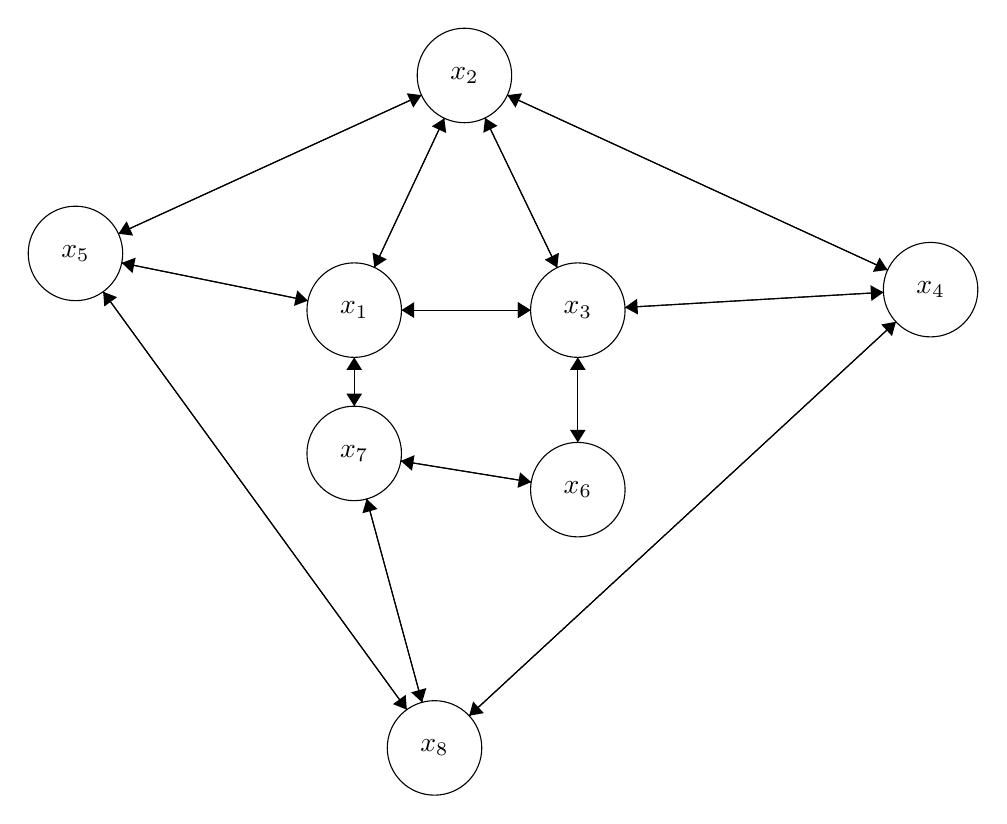
\begin{tikzpicture}[scale=0.2]
\tikzstyle{every node}+=[inner sep=0pt]
\draw [black] (17.6,-20.2) circle (3);
\draw (17.6,-20.2) node {$x_5$};
\draw [black] (42.3,-8.9) circle (3);
\draw (42.3,-8.9) node {$x_2$};
\draw [black] (71.9,-22.5) circle (3);
\draw (71.9,-22.5) node {$x_4$};
\draw [black] (49.5,-23.8) circle (3);
\draw (49.5,-23.8) node {$x_3$};
\draw [black] (35.3,-23.8) circle (3);
\draw (35.3,-23.8) node {$x_1$};
\draw [black] (49.5,-35.2) circle (3);
\draw (49.5,-35.2) node {$x_6$};
\draw [black] (35.3,-32.9) circle (3);
\draw (35.3,-32.9) node {$x_7$};
\draw [black] (40.4,-51.6) circle (3);
\draw (40.4,-51.6) node {$x_8$};
\draw [black] (20.33,-18.95) -- (39.57,-10.15);
\fill [black] (39.57,-10.15) -- (38.64,-10.03) -- (39.05,-10.94);
\draw [black] (39.57,-10.15) -- (20.33,-18.95);
\fill [black] (20.33,-18.95) -- (21.26,-19.07) -- (20.85,-18.16);
\draw [black] (41.02,-11.62) -- (36.58,-21.08);
\fill [black] (36.58,-21.08) -- (37.37,-20.57) -- (36.46,-20.15);
\draw [black] (36.58,-21.08) -- (41.02,-11.62);
\fill [black] (41.02,-11.62) -- (40.23,-12.13) -- (41.14,-12.55);
\draw [black] (48.19,-21.1) -- (43.61,-11.6);
\fill [black] (43.61,-11.6) -- (43.5,-12.54) -- (44.4,-12.1);
\draw [black] (43.61,-11.6) -- (48.19,-21.1);
\fill [black] (48.19,-21.1) -- (48.3,-20.16) -- (47.4,-20.6);
\draw [black] (45.03,-10.15) -- (69.17,-21.25);
\fill [black] (69.17,-21.25) -- (68.66,-20.46) -- (68.24,-21.37);
\draw [black] (69.17,-21.25) -- (45.03,-10.15);
\fill [black] (45.03,-10.15) -- (45.54,-10.94) -- (45.96,-10.03);
\draw [black] (19.36,-22.63) -- (38.64,-49.17);
\fill [black] (38.64,-49.17) -- (38.57,-48.23) -- (37.76,-48.82);
\draw [black] (38.64,-49.17) -- (19.36,-22.63);
\fill [black] (19.36,-22.63) -- (19.43,-23.57) -- (20.24,-22.98);
\draw [black] (42.6,-49.56) -- (69.7,-24.54);
\fill [black] (69.7,-24.54) -- (68.77,-24.71) -- (69.45,-25.45);
\draw [black] (69.7,-24.54) -- (42.6,-49.56);
\fill [black] (42.6,-49.56) -- (43.53,-49.39) -- (42.85,-48.65);
\draw [black] (49.5,-32.2) -- (49.5,-26.8);
\fill [black] (49.5,-26.8) -- (49,-27.6) -- (50,-27.6);
\draw [black] (49.5,-26.8) -- (49.5,-32.2);
\fill [black] (49.5,-32.2) -- (50,-31.4) -- (49,-31.4);
\draw [black] (38.3,-23.8) -- (46.5,-23.8);
\fill [black] (46.5,-23.8) -- (45.7,-23.3) -- (45.7,-24.3);
\draw [black] (38.3,-23.8) -- (46.5,-23.8);
\fill [black] (46.5,-23.8) -- (45.7,-23.3) -- (45.7,-24.3);
\draw [black] (46.5,-23.8) -- (38.3,-23.8);
\fill [black] (38.3,-23.8) -- (39.1,-24.3) -- (39.1,-23.3);
\draw [black] (35.3,-26.8) -- (35.3,-29.9);
\fill [black] (35.3,-29.9) -- (35.8,-29.1) -- (34.8,-29.1);
\draw [black] (35.3,-29.9) -- (35.3,-26.8);
\fill [black] (35.3,-26.8) -- (34.8,-27.6) -- (35.8,-27.6);
\draw [black] (38.26,-33.38) -- (46.54,-34.72);
\fill [black] (46.54,-34.72) -- (45.83,-34.1) -- (45.67,-35.09);
\draw [black] (46.54,-34.72) -- (38.26,-33.38);
\fill [black] (38.26,-33.38) -- (38.97,-34) -- (39.13,-33.01);
\draw [black] (36.09,-35.79) -- (39.61,-48.71);
\fill [black] (39.61,-48.71) -- (39.88,-47.8) -- (38.92,-48.07);
\draw [black] (39.61,-48.71) -- (36.09,-35.79);
\fill [black] (36.09,-35.79) -- (35.82,-36.7) -- (36.78,-36.43);
\draw [black] (52.49,-23.63) -- (68.91,-22.67);
\fill [black] (68.91,-22.67) -- (68.08,-22.22) -- (68.14,-23.22);
\draw [black] (68.91,-22.67) -- (52.49,-23.63);
\fill [black] (52.49,-23.63) -- (53.32,-24.08) -- (53.26,-23.08);
\draw [black] (20.54,-20.8) -- (32.36,-23.2);
\fill [black] (32.36,-23.2) -- (31.68,-22.55) -- (31.48,-23.53);
\draw [black] (32.36,-23.2) -- (20.54,-20.8);
\fill [black] (20.54,-20.8) -- (21.22,-21.45) -- (21.42,-20.47);
\end{tikzpicture}
\end{center}
\newpage
Graf G3:

\begin{center}
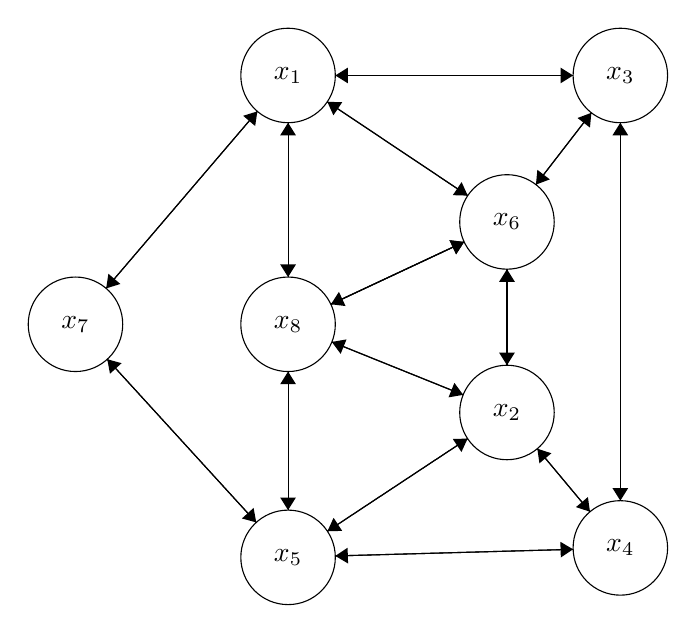
\begin{tikzpicture}[scale=0.2]
\tikzstyle{every node}+=[inner sep=0pt]
\draw [black] (30.5,-32.4) circle (3);
\draw (30.5,-32.4) node {$x_8$};
\draw [black] (44.4,-38) circle (3);
\draw (44.4,-38) node {$x_2$};
\draw [black] (51.6,-46.6) circle (3);
\draw (51.6,-46.6) node {$x_4$};
\draw [black] (51.6,-16.6) circle (3);
\draw (51.6,-16.6) node {$x_3$};
\draw [black] (30.5,-16.6) circle (3);
\draw (30.5,-16.6) node {$x_1$};
\draw [black] (44.4,-25.9) circle (3);
\draw (44.4,-25.9) node {$x_6$};
\draw [black] (17,-32.4) circle (3);
\draw (17,-32.4) node {$x_7$};
\draw [black] (30.5,-47.2) circle (3);
\draw (30.5,-47.2) node {$x_5$};
\draw [black] (33.5,-16.6) -- (48.6,-16.6);
\fill [black] (48.6,-16.6) -- (47.8,-16.1) -- (47.8,-17.1);
\draw [black] (48.6,-16.6) -- (33.5,-16.6);
\fill [black] (33.5,-16.6) -- (34.3,-17.1) -- (34.3,-16.1);
\draw [black] (46.24,-23.53) -- (49.76,-18.97);
\fill [black] (49.76,-18.97) -- (48.88,-19.3) -- (49.67,-19.91);
\draw [black] (49.76,-18.97) -- (46.24,-23.53);
\fill [black] (46.24,-23.53) -- (47.12,-23.2) -- (46.33,-22.59);
\draw [black] (41.91,-24.23) -- (32.99,-18.27);
\fill [black] (32.99,-18.27) -- (33.38,-19.13) -- (33.94,-18.3);
\draw [black] (32.99,-18.27) -- (41.91,-24.23);
\fill [black] (41.91,-24.23) -- (41.52,-23.37) -- (40.96,-24.2);
\draw [black] (44.4,-28.9) -- (44.4,-35);
\fill [black] (44.4,-35) -- (44.9,-34.2) -- (43.9,-34.2);
\draw [black] (44.4,-35) -- (44.4,-28.9);
\fill [black] (44.4,-28.9) -- (43.9,-29.7) -- (44.9,-29.7);
\draw [black] (51.6,-43.6) -- (51.6,-19.6);
\fill [black] (51.6,-19.6) -- (51.1,-20.4) -- (52.1,-20.4);
\draw [black] (51.6,-19.6) -- (51.6,-43.6);
\fill [black] (51.6,-43.6) -- (52.1,-42.8) -- (51.1,-42.8);
\draw [black] (49.67,-44.3) -- (46.33,-40.3);
\fill [black] (46.33,-40.3) -- (46.46,-41.23) -- (47.22,-40.59);
\draw [black] (46.33,-40.3) -- (49.67,-44.3);
\fill [black] (49.67,-44.3) -- (49.54,-43.37) -- (48.78,-44.01);
\draw [black] (48.6,-46.69) -- (33.5,-47.11);
\fill [black] (33.5,-47.11) -- (34.31,-47.59) -- (34.28,-46.59);
\draw [black] (33,-45.54) -- (41.9,-39.66);
\fill [black] (41.9,-39.66) -- (40.96,-39.68) -- (41.51,-40.51);
\draw [black] (33.5,-47.11) -- (48.6,-46.69);
\fill [black] (48.6,-46.69) -- (47.79,-46.21) -- (47.82,-47.21);
\draw [black] (41.9,-39.66) -- (33,-45.54);
\fill [black] (33,-45.54) -- (33.94,-45.52) -- (33.39,-44.69);
\draw [black] (33.22,-31.13) -- (41.68,-27.17);
\fill [black] (41.68,-27.17) -- (40.75,-27.06) -- (41.17,-27.96);
\draw [black] (41.62,-36.88) -- (33.28,-33.52);
\fill [black] (33.28,-33.52) -- (33.84,-34.28) -- (34.21,-33.36);
\draw [black] (33.22,-31.13) -- (41.68,-27.17);
\fill [black] (41.68,-27.17) -- (40.75,-27.06) -- (41.17,-27.96);
\draw [black] (41.68,-27.17) -- (33.22,-31.13);
\fill [black] (33.22,-31.13) -- (34.15,-31.24) -- (33.73,-30.34);
\draw [black] (33.28,-33.52) -- (41.62,-36.88);
\fill [black] (41.62,-36.88) -- (41.06,-36.12) -- (40.69,-37.04);
\draw [black] (30.5,-29.4) -- (30.5,-19.6);
\fill [black] (30.5,-19.6) -- (30,-20.4) -- (31,-20.4);
\draw [black] (30.5,-19.6) -- (30.5,-29.4);
\fill [black] (30.5,-29.4) -- (31,-28.6) -- (30,-28.6);
\draw [black] (30.5,-44.2) -- (30.5,-35.4);
\fill [black] (30.5,-35.4) -- (30,-36.2) -- (31,-36.2);
\draw [black] (30.5,-35.4) -- (30.5,-44.2);
\fill [black] (30.5,-44.2) -- (31,-43.4) -- (30,-43.4);
\draw [black] (28.55,-18.88) -- (18.95,-30.12);
\fill [black] (18.95,-30.12) -- (19.85,-29.84) -- (19.09,-29.19);
\draw [black] (18.95,-30.12) -- (28.55,-18.88);
\fill [black] (28.55,-18.88) -- (27.65,-19.16) -- (28.41,-19.81);
\draw [black] (19.02,-34.62) -- (28.48,-44.98);
\fill [black] (28.48,-44.98) -- (28.31,-44.06) -- (27.57,-44.73);
\draw [black] (28.48,-44.98) -- (19.02,-34.62);
\fill [black] (19.02,-34.62) -- (19.19,-35.54) -- (19.93,-34.87);
\end{tikzpicture}
\end{center}

Graf G2 nije planaran jer kontrakcijom ivica dobijamo graf K5, tj. prema Wagnerovoj teoremi, nije planaran.

d)

Za graf G1:

$$x1 \rightarrow 4$$
$$x2 \rightarrow 1$$
$$x3 \rightarrow 2$$
$$x4 \rightarrow 3$$
$$x5 \rightarrow 2$$
$$x6 \rightarrow 1$$
$$x7 \rightarrow 3$$
$$x8 \rightarrow 1$$

Za graf G2:

$$x1 \rightarrow 1$$
$$x2 \rightarrow 2$$
$$x3 \rightarrow 3$$
$$x4 \rightarrow 1$$
$$x5 \rightarrow 3$$
$$x6 \rightarrow 2$$
$$x7 \rightarrow 1$$
$$x8 \rightarrow 3$$

Za graf G3:

$$x1 \rightarrow 4$$
$$x2 \rightarrow 1$$
$$x3 \rightarrow 1$$
$$x4 \rightarrow 2$$
$$x5 \rightarrow 3$$
$$x6 \rightarrow 3$$
$$x7 \rightarrow 1$$
$$x8 \rightarrow 2$$


\newpage
\section*{Zadatak 2\label{Z2}}

\underline{Postavka:}

Potrebno je povezati 12 lokacija L1 – L12 u računarsku mrežu. Zbog tehnoloških ograničenja, kablove nije moguće razvesti između proizvoljne dvije lokacije. Sljedeći spisak opisuje sve moguće načine kablovskog povezivanja lokacija, pri čemu trojka oblika (Li, Lj, dij) označava da je moguće spojiti lokacije Li i Lj, i to kablom dužine dij (u metrima): 

(L1, L3, 360)   (L1, L5, 1240)   (L1, L7, 1290)   (L2, L6, 410)   (L2, L9, 1400)   (L2, L10, 370)   (L2, L11, 400)   (L2, L12, 390)   (L3, L4, 280)   (L3, L9, 480)   (L3, L11, 640)   (L4, L7, 450)   (L4, L9, 1200)   (L4, L11, 1320)   (L5, L6, 350)   (L5, L8, 810)   (L5, L9, 680)   (L6, L8, 580)   (L6, L9, 750)   (L6, L10, 300)   (L6, L11, 1260)   (L7, L9, 740)   (L8, L12, 1020)   (L9, L12, 1000)   (L10, L12, 1190)   


Dizajnirajte računarsku mrežu u skladu sa navedenim specifikacijama tako da ukupan utrošak kablova bude minimalan i obavezno naznačite koliko iznosi taj utrošak. Dizajn obavite

Primjenom Kruskalovog algoritma sa bojenjem čvorova;

Primjenom optimalnog Kruskalovog algoritma;

Primjenom optimiziranog (kvadratnog) Primovog algoritma.


U sva tri slučaja, nemojte crtati odgovarajući graf, nego sve neophodne radnje obavljajte “naslijepo”, koristeći samo raspoložive podatke, eventualno uz bilježenje izvjesnih pomoćnih informacija.

\underline{Rješenje:}
\newpage

U koloni Grana smo izostavili 'L', ali se podrazumijeva.

a) Kruskalov algoritam


\begin{table}[hp]
\centering
\begin{tabular}{|l|l|l|l|l|l|l|l|l|l|l|l|l|l|l|}
\hline
Grana  & Težina & Uzeti & c1 & c2 & c3 & c4 & c5 & c6 & c7 & c8 & c9 & c10 & c11 & c12 \\ \hline
3, 4   & 280    & da    &    &    & 1  & 1  &    &    &    &    &    &     &     &     \\ \hline
6, 10  & 300    & da    &    &    &    &    &    & 2  &    &    &    & 2   &     &     \\ \hline
5, 6   & 350    & da    &    &    &    &    & 2  &    &    &    &    &     &     &     \\ \hline
1, 3   & 360    & da    & 1  &    &    &    &    &    &    &    &    &     &     &     \\ \hline
2, 10  & 370    & da    &    & 2  &    &    &    &    &    &    &    &     &     &     \\ \hline
2, 12  & 390    & da    &    &    &    &    &    &    &    &    &    &     &     & 2   \\ \hline
2, 11  & 400    & da    &    &    &    &    &    &    &    &    &    &     & 2   &     \\ \hline
2, 6   & 410    & ne    &    &    &    &    &    &    &    &    &    &     &     &     \\ \hline
4, 7   & 450    & da    &    &    &    &    &    &    & 1  &    &    &     &     &     \\ \hline
3, 9   & 480    & da    &    &    &    &    &    &    &    &    & 1  &     &     &     \\ \hline
6, 8   & 580    & da    &    &    &    &    &    &    &    & 2  &    &     &     &     \\ \hline
3, 11  & 640    & da    &    & 1  & 1  &    & 1  & 1  &    & 1  &    & 1   & 1   & 1   \\ \hline
5, 9   & 680    & ne    &    &    &    &    &    &    &    &    &    &     &     &     \\ \hline
7, 9   & 740    & ne    &    &    &    &    &    &    &    &    &    &     &     &     \\ \hline
6, 9   & 750    & ne    &    &    &    &    &    &    &    &    &    &     &     &     \\ \hline
5, 8   & 810    & ne    &    &    &    &    &    &    &    &    &    &     &     &     \\ \hline
9, 12  & 1000   & ne    &    &    &    &    &    &    &    &    &    &     &     &     \\ \hline
8, 12  & 1020   & ne    &    &    &    &    &    &    &    &    &    &     &     &     \\ \hline
10, 12 & 1190   & ne    &    &    &    &    &    &    &    &    &    &     &     &     \\ \hline
4, 9   & 1200   & ne    &    &    &    &    &    &    &    &    &    &     &     &     \\ \hline
1, 5   & 1240   & ne    &    &    &    &    &    &    &    &    &    &     &     &     \\ \hline
6, 11  & 1240   & ne    &    &    &    &    &    &    &    &    &    &     &     &     \\ \hline
1, 7   & 1290   & ne    &    &    &    &    &    &    &    &    &    &     &     &     \\ \hline
4, 11  & 1320   & ne    &    &    &    &    &    &    &    &    &    &     &     &     \\ \hline
2, 9   & 1400   & ne    &    &    &    &    &    &    &    &    &    &     &     &     \\ \hline
\end{tabular}
\end{table}
T =  \{ (\(L_{3}\), \(L_{4}\), 280), (\(L_{10}\), \(L_{6}\), 300), (\(L_{5}\), \(L_{6}\), 350), (\(L_{1}\), \(L_{3}\), 360), (\(L_{2}\), \(L_{10}\), 370), (\(L_{2}\), \(L_{12}\), 390), (\(L_{2}\), \(L_{11}\), 400), (\(L_{4}\), \(L_{7}\), 450), (\(L_{9}\), \(L_{3}\), 480), (\(L_{8}\), \(L_{6}\), 580), (\(L_{3}\), \(L_{11}\), 640) \}

Suma svih težina je 4600.


\newpage
b) Optimalni Kruskalov algoritam


\begin{table}[hp]
\centering
\hspace*{-1.3in}
\begin{tabular}{|l|l|l|l|l|l|l|l|l|l|l|l|l|l|l|}
\hline
Grana  & Težina & Uzeti & x1/1 & x2/1 & x3/1 & x4/1 & x5/1 & x6/1  & x7/1 & x8/1 & x9/1 & x10/1 & x11/1 & x12/1 \\ \hline
3, 4   & 280    & da    &      &      & x3/2 & x3/1 &      &       &      &      &      &       &       &       \\ \hline
6, 10  & 300    & da    &      &      &      &      &      & x6/2  &      &      &      & x6/1  &       &       \\ \hline
5, 6   & 350    & da    &      &      &      &      & x6/1 & x6/3  &      &      &      &       &       &       \\ \hline
1, 3   & 360    & da    & x1/1 &      & x3/3 &      &      &       &      &      &      &       &       &       \\ \hline
2, 10  & 370    & da    &      & x6/1 &      &      &      & x6/4  &      &      &      &       &       &       \\ \hline
2, 12  & 390    & da    &      &      &      &      &      & x6/5  &      &      &      &       &       & x6/1  \\ \hline
2, 11  & 400    & da    &      &      &      &      &      & x6/6  &      &      &      &       & x6/1  &       \\ \hline
2, 6   & 410    & ne    &      &      &      &      &      &       &      &      &      &       &       &       \\ \hline
4, 7   & 450    & da    &      &      & x3/4 &      &      &       & x3/1 &      &      &       &       &       \\ \hline
3, 9   & 480    & da    &      &      & x3/5 &      &      &       &      &      & x3/1 &       &       &       \\ \hline
6, 8   & 580    & da    &      &      &      &      &      & x6/7  &      & x6/1 &      &       &       &       \\ \hline
3, 11  & 640    & da    &      &      & x6/4 &      &      & x6/11 &      &      &      &       &       &       \\ \hline
5, 9   & 680    & ne    &      &      &      &      &      &       &      &      &      &       &       &       \\ \hline
7, 9   & 740    & ne    &      &      &      &      &      &       &      &      &      &       &       &       \\ \hline
6, 9   & 750    & ne    &      &      &      &      &      &       &      &      &      &       &       &       \\ \hline
5, 8   & 810    & ne    &      &      &      &      &      &       &      &      &      &       &       &       \\ \hline
9, 12  & 1000   & ne    &      &      &      &      &      &       &      &      &      &       &       &       \\ \hline
8, 12  & 1020   & ne    &      &      &      &      &      &       &      &      &      &       &       &       \\ \hline
10, 12 & 1190   & ne    &      &      &      &      &      &       &      &      &      &       &       &       \\ \hline
4, 9   & 1200   & ne    &      &      &      &      &      &       &      &      &      &       &       &       \\ \hline
1, 5   & 1240   & ne    &      &      &      &      &      &       &      &      &      &       &       &       \\ \hline
6, 11  & 1240   & ne    &      &      &      &      &      &       &      &      &      &       &       &       \\ \hline
1, 7   & 1290   & ne    &      &      &      &      &      &       &      &      &      &       &       &       \\ \hline
4, 11  & 1320   & ne    &      &      &      &      &      &       &      &      &      &       &       &       \\ \hline
2, 9   & 1400   & ne    &      &      &      &      &      &       &      &      &      &       &       &       \\ \hline
\end{tabular}
\end{table}
T =  \{ (\(L_{3}\), \(L_{4}\), 280), (\(L_{10}\), \(L_{6}\), 300), (\(L_{5}\), \(L_{6}\), 350), (\(L_{1}\), \(L_{3}\), 360), (\(L_{2}\), \(L_{10}\), 370), (\(L_{2}\), \(L_{12}\), 390), (\(L_{2}\), \(L_{11}\), 400), (\(L_{4}\), \(L_{7}\), 450), (\(L_{9}\), \(L_{3}\), 480), (\(L_{8}\), \(L_{6}\), 580), (\(L_{3}\), \(L_{11}\), 640) \}

Suma svih težina je 4600.
\newpage
c) Optimizirani kvadratni Primov algoritam

Primjetimo da u tabeli oznake čvorova ne idu od L1 nego L10 - L12, te L1 - L9

\begin{tabular}{ | c || c  | c | c | c | c | c | c | c | c | c | c | c | }
\hline
Iteracija & \(L_{10}\) & \(L_{11}\) & \(L_{12}\) & \(L_{1}\) & \(L_{2}\) & \(L_{3}\) & \(L_{4}\) & \(L_{5}\) & \(L_{6}\) & \(L_{7}\) & \(L_{8}\) & \(L_{9}\)\\
 \hline
 \hline
Pocetno stanje & $\infty$ & $\infty$ & $\infty$ & $\infty$ & $\infty$ & $\infty$ & $\infty$ & $\infty$ & $\infty$ & $\infty$ & $\infty$ & $\infty$\\
 \hline
(\(L_{10}\), \(L_{10}\), 0) & 0 & $\infty$ & 1190 & $\infty$ & 370 & $\infty$ & $\infty$ & $\infty$ & 300 & $\infty$ & $\infty$ & $\infty$\\
 \hline
(\(L_{10}\), \(L_{6}\), 300) & 0 & 1260 & 1190 & $\infty$ & 370 & $\infty$ & $\infty$ & 350 & 300 & $\infty$ & 580 & 750\\
 \hline
(\(L_{6}\), \(L_{5}\), 350) & 0 & 1260 & 1190 & 1240 & 370 & $\infty$ & $\infty$ & 350 & 300 & $\infty$ & 580 & 680\\
 \hline
(\(L_{10}\), \(L_{2}\), 370) & 0 & 400 & 390 & 1240 & 370 & $\infty$ & $\infty$ & 350 & 300 & $\infty$ & 580 & 680\\
 \hline
(\(L_{2}\), \(L_{12}\), 390) & 0 & 400 & 390 & 1240 & 370 & $\infty$ & $\infty$ & 350 & 300 & $\infty$ & 580 & 680\\
 \hline
(\(L_{2}\), \(L_{11}\), 400) & 0 & 400 & 390 & 1240 & 370 & 640 & 1320 & 350 & 300 & $\infty$ & 580 & 680\\
 \hline
(\(L_{6}\), \(L_{8}\), 580) & 0 & 400 & 390 & 1240 & 370 & 640 & 1320 & 350 & 300 & $\infty$ & 580 & 680\\
 \hline
(\(L_{11}\), \(L_{3}\), 640) & 0 & 400 & 390 & 360 & 370 & 640 & 280 & 350 & 300 & $\infty$ & 580 & 480\\
 \hline
(\(L_{3}\), \(L_{4}\), 280) & 0 & 400 & 390 & 360 & 370 & 640 & 280 & 350 & 300 & 450 & 580 & 480\\
 \hline
(\(L_{3}\), \(L_{1}\), 360) & 0 & 400 & 390 & 360 & 370 & 640 & 280 & 350 & 300 & 450 & 580 & 480\\
 \hline
(\(L_{4}\), \(L_{7}\), 450) & 0 & 400 & 390 & 360 & 370 & 640 & 280 & 350 & 300 & 450 & 580 & 480\\
 \hline
(\(L_{3}\), \(L_{9}\), 480) & 0 & 400 & 390 & 360 & 370 & 640 & 280 & 350 & 300 & 450 & 580 & 480\\
 \hline
\end{tabular}


T =  \{ (\(L_{10}\), \(L_{6}\), 300), (\(L_{6}\), \(L_{5}\), 350), (\(L_{10}\), \(L_{2}\), 370), (\(L_{2}\), \(L_{12}\), 390), (\(L_{2}\), \(L_{11}\), 400), (\(L_{6}\), \(L_{8}\), 580), (\(L_{11}\), \(L_{3}\), 640), (\(L_{3}\), \(L_{4}\), 280), (\(L_{3}\), \(L_{1}\), 360), (\(L_{4}\), \(L_{7}\), 450), (\(L_{3}\), \(L_{9}\), 480) \}

Suma svih težina je 4600.
\newpage
\section*{Zadatak 3\label{Z3}}
\underline{Postavka:}

Turistička agencija “Pljačkaš tours” ima poslovnice u 8 gradova: Amcazo, Uhsuru, Quwuti, Brot, Zixa, Sosyab, Xanu i Urasoto. U sljedećoj tablici su date cijene direktnih avionskih letova između pojedinih gradova izražene u škafiškafnjacima (crtica znači da direktan let ne postoji):

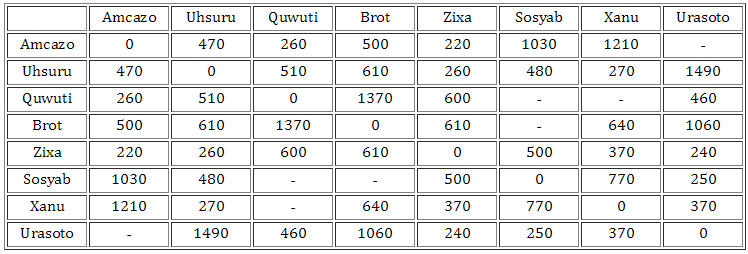
\includegraphics[width=\linewidth]{table.PNG}
\\
Međutim, poznato je da direktni letovi nisu uvijek i najjeftiniji način aviotransporta između gradova, nego je nekada povoljnije koristiti presjedanje (pogotovo ako se na taj način mogu koristiti usluge low-cost kompanija. Na primjer, iz Quwutija jeftinije je u Brot putovati sa presjedanjem u Uhsuruu nego direktnim letom (sa presjedanjem plaćamo 510 + 610 = 1120 škafiškafnjaka, dok direktan let košta 1370 škafiškafnjaka). Zbog toga, turistička agencija želi da sastavi tablicu koja sadrži informacije koliko iznose najjeftinije cijene aviotransporta između svakog para gradova u kojima agencija ima poslovnice (uz dopuštanje presjedanja) kao i u kojim gradovima treba eventualno vršiti presjedanja za svaki od tih transporta. Pomozite agenciji “Pljačkaš tours” da sastavi ove tablice. Postupak obavite uz pomoć Dijkstrinog algoritma, ali bez crtanja grafova, nego samo vršeći manipulacije nad zadanom tablicom, uz eventualno bilježenje pomoćnih dopunskih informacija.


\underline{Rješenje:}
\newpage

Pokazat ćemo Dijkstrin algoritam za 2 tabele tj. 2 grada, ostale tabele se rade analogno. Potrebno je minimalno 7 tabela(7 razlicitih gradova) da bi se dobile sve potrebne informacije. Rješenje ćemo predstaviti također u vidu tabele.

Kodirati ćemo gradove tako da ih je lakše predstaviti:

Amcazo - A, Uhsuru - B, Quwuti - C, Brot - D, Zixa - E, Sosyab - F, Xanu - G, Urasoto - H

Za Amcazo:

\begin{table}[hp]
\centering
\begin{tabular}{|l|l|l|l|l|l|l|l|l|}
\hline
             & A & B     & C     & D       & E       & F      & G        & H  \\ \hline
             & 0      & -          & -          & -          & -          & -           & -           & -        \\ \hline
A(0)    &        & 470/A & 260/A & 500/A & 220/A & 1030/A & 1210/A & -        \\ \hline
E(220)    &        & 470/A & 260/A & 500/A &            & 720/E    & 590/E    & 460/E \\ \hline
C(460)  &        & 470/A &            & 500/A &            & 720/E    & 590/E    & 460/E \\ \hline
H(460) &        & 470/A &            & 500/A &            & 710/H & 590/E    &          \\ \hline
B(470)  &        &            &            & 500/A &            & 710/H & 590/E    &          \\ \hline
D(500)    &        &            &            &            &            & 710/H & 590/E    &          \\ \hline
G(590)    &        &            &            &            &            & 710/H &             &          \\ \hline
F(710)  &        &            &            &            &            &             &             &          \\ \hline
\end{tabular}
\end{table}

Za Uhsuru

\begin{table}[hp]
\centering
\begin{tabular}{|l|l|l|l|l|l|l|l|l|}
\hline
       & A     & B & C     & D     & E     & F     & G     & H      \\ \hline
       & -     & 0 & -     & -     & -     & -     & -     & -      \\ \hline
B(0)   & 470/B &   & 510/B & 610/B & 260/B & 480/B & 270/B & 1490/B \\ \hline
E(260) & 470/B &   & 510/B & 610/B &       & 480/B & 270/B & 500/E  \\ \hline
G(270) & 470/B &   & 510/B & 610/B &       & 480/B &       & 500/E  \\ \hline
A(470) &       &   & 510/B & 610/B &       & 480/B &       & 500/E  \\ \hline
F(480) &       &   & 510/B & 610/B &       &       &       & 500/E  \\ \hline
H(500) &       &   & 510/B & 610/B &       &       &       &        \\ \hline
C(510) &       &   &       & 610/B &       &       &       &        \\ \hline
D(610) &       &   &       &       &       &       &       &        \\ \hline
\end{tabular}
\end{table}
\newpage
Itd. za gradove C - G. Konačno se dobije:

\begin{table}[hp]
\centering
\begin{tabular}{|l|l|l|l|l|l|l|l|l|}
\hline
 & Amcazo & Uhsuru & Quwuti & Brot & Zixa & Sosyab & Xanu & Urasoto \\ \hline
Amcazo & 0 & 470 & 260 & 500 & 220 & 710 & 590 & 460 \\ \hline
Uhsuru & 470 & 0 & 510 & 610 & 260 & 480 & 270 & 500 \\ \hline
Quwuti & 260 & 510 & 0 & 760 & 480 & 710 & 780 & 460 \\ \hline
Brot & 500 & 610 & 760 & 0 & 610 & 1090 & 640 & 850 \\ \hline
Zixa & 220 & 260 & 480 & 610 & 0 & 490 & 370 & 240 \\ \hline
Sosyab & 710 & 480 & 710 & 1090 & 490 & 0 & 620 & 250 \\ \hline
Xanu & 590 & 270 & 780 & 640 & 370 & 620 & 0 & 370 \\ \hline
Urasoto & 460 & 500 & 460 & 850 & 240 & 250 & 370 & 0 \\ \hline
\end{tabular}
\end{table}

\newpage

\section*{Zadatak 4\label{Z4}}
\underline{Postavka:}

Dat je usmjereni težinski graf

$$G = \{\{A, B, C, D, E, F, G, H, I, J\}, \{(A, I, 65), (B, G, -95), (C, D, 65), (C, F, 55),$$
 $$(C, I, 75), (D, A, -105), (D, H, 60), (E, H, 70), (F, D, 80), (F, E, -65), $$
$$(G, A, 40), (G, C, -30), (G, E, 50), (H, B, 45), (H, G, 60),$$
$$(I, H, 20), (J, C, -85), (J, D, 25)\}\}$$

Koristeći Bellman-Fordov algoritam, dokažite da u ovom grafu postoji kontura sa negativnom sumom težina u konturi. Nakon toga pronađite makar jednu takvu konturu. Postupak obavite “naslijepo”, bez crtanja grafa, koristeći samo raspoložive informacije (eventualno uz bilježenje raznih pomoćnih informacija).


\underline{Rješenje:}

Dovoljno je da pokažemo da suma grana u konturi kojoj pripada prvi čvor tj. čvor A bude $\lambda_A < 0$.
Pokazuje se da je za konrektan problem dovoljno 4 iteracije da bi se dobio traženi uslov.

Iteracija1:

\begin{table}[hp]
\centering
\begin{tabular}{|l|l|l|l|l|l|l|l|l|l|l|l|}
\hline
\multirow{2}{*}{} & A & B & C & D & E & F & G & H & I & J & \multirow{2}{*}{$\lambda$} \\ \cline{2-11}
 & 0 & $\infty$ & $\infty$ & $\infty$ & $\infty$ & $\infty$ & $\infty$ & $\infty$ & $\infty$ & $\infty$ &  \\ \hline
A &  &  &  &  &  &  &  &  & 65 &  & $\infty$ \\ \hline
B &  &  &  &  &  &  &  &  &  &  & $\infty$ \\ \hline
C &  &  &  &  &  &  &  &  &  &  & $\infty$ \\ \hline
D &  &  &  &  &  &  &  &  &  &  & $\infty$ \\ \hline
E &  &  &  &  &  &  &  &  &  &  & $\infty$ \\ \hline
F &  &  &  &  &  &  &  &  &  &  & $\infty$ \\ \hline
G &  &  &  &  &  &  &  &  &  &  & $\infty$ \\ \hline
H &  &  &  &  &  &  &  &  &  &  & $\infty$, 85 \\ \hline
I &  &  &  &  &  &  &  & 85 &  &  & $\infty$, 65 \\ \hline
J &  &  &  &  &  &  &  &  &  &  & $\infty$ \\ \hline
\end{tabular}
\end{table}
\newpage
Iteracija2:

\begin{table}[hp]
\centering
\begin{tabular}{|l|l|l|l|l|l|l|l|l|l|l|l|}
\hline
\multirow{2}{*}{} & A & B & C & D & E & F & G & H & I & J & \multirow{2}{*}{$\lambda$} \\ \cline{2-11}
 & 0 & $\infty$ & $\infty$ & $\infty$ & $\infty$ & $\infty$ & $\infty$ & 85 & 65 & $\infty$ &  \\ \hline
A &  &  &  &  &  &  &  &  &  &  & $\infty$ \\ \hline
B &  &  &  &  &  &  &  &  &  &  & $\infty$, 130 \\ \hline
C &  &  &  &  &  &  &  &  &  &  & $\infty$ \\ \hline
D &  &  &  &  &  &  &  &  &  &  & $\infty$ \\ \hline
E &  &  &  &  &  &  &  &  &  &  & $\infty$ \\ \hline
F &  &  &  &  &  &  &  &  &  &  & $\infty$ \\ \hline
G &  &  &  &  &  &  &  &  &  &  & $\infty$, 145 \\ \hline
H &  & 130 &  &  &  &  & 145 &  &  &  & 85 \\ \hline
I &  &  &  &  &  &  &  &  &  &  & 65 \\ \hline
J &  &  &  &  &  &  &  &  &  &  & $\infty$ \\ \hline
\end{tabular}
\end{table}

Iteracija 3:

\begin{table}[hp]
\centering
\begin{tabular}{|l|l|l|l|l|l|l|l|l|l|l|l|}
\hline
\multirow{2}{*}{} & A & B & C & D & E & F & G & H & I & J & \multirow{2}{*}{$\lambda$} \\ \cline{2-11}
 & 0 & 130 & $\infty$ & $\infty$ & $\infty$ & $\infty$ & 145 & 85 & 65 & $\infty$ &  \\ \hline
A &  &  &  &  &  &  &  &  &  &  & $\infty$ \\ \hline
B &  &  &  &  &  &  & 35 &  &  &  & 130 \\ \hline
C &  &  &  &  &  &  &  &  &  &  & $\infty$, 5 \\ \hline
D &  &  &  &  &  &  &  &  &  &  & $\infty$ \\ \hline
E &  &  &  &  &  &  &  &  &  &  & $\infty$, 85 \\ \hline
F &  &  &  &  &  &  &  &  &  &  & $\infty$ \\ \hline
G &  &  & 5 &  & 85 &  &  &  &  &  & 145, 35 \\ \hline
H &  &  &  &  &  &  &  &  &  &  & 85 \\ \hline
I &  &  &  &  &  &  &  &  &  &  & 65 \\ \hline
J &  &  &  &  &  &  &  &  &  &  & $\infty$ \\ \hline
\end{tabular}
\end{table}
\newpage
Iteracija 4:

\begin{table}[hp]
\centering
\begin{tabular}{|l|l|l|l|l|l|l|l|l|l|l|l|}
\hline
\multirow{2}{*}{} & A & B & C & D & E & F & G & H & I & J & \multirow{2}{*}{$\lambda$} \\ \cline{2-11}
 & 0 & 130 & 5 & $\infty$ & 85 & $\infty$ & 35 & 85 & 65 & $\infty$ &  \\ \hline
A &  &  &  &  &  &  &  &  &  &  & 0, -35 \\ \hline
B &  &  &  &  &  &  &  &  &  &  & 130 \\ \hline
C &  &  &  & 70 &  & 60 &  &  &  &  & 5 \\ \hline
D & -35 &  &  &  &  &  &  &  &  &  & $\infty$. 70 \\ \hline
E &  &  &  &  &  &  &  & 65 &  &  & 85, -5 \\ \hline
F &  &  &  & 140 & -5 &  &  &  &  &  & $\infty$, 60 \\ \hline
G &  &  &  &  &  &  &  &  &  &  & 35 \\ \hline
\end{tabular}
\end{table}

Dobili smo $\lambda_A = -35 < 0$, pa je pronađen put negativne dužine koji spaja čvor A sam sa sobom. Algoritam sigurno neće terminirati. Dakle, kontura sa negativnom sumom težina je: A-I-H-B-G-C-D-A.






























































\end{document}